\documentclass{report}
\usepackage[utf8]{inputenc}
\usepackage[T1]{fontenc}
\usepackage{indentfirst}
\usepackage{fancyhdr}
\usepackage[french]{babel}
\setlength{\textwidth}{155mm}
\setlength{\textheight}{255mm}
%\setlength{\evensidemargin}{0mm}
%\setlength{\oddsidemargin}{5mm}
\setlength{\headheight}{0mm}
\setlength{\headsep}{0mm}
\setlength{\topmargin}{-10mm}
\renewcommand{\contentsname}{\hspace*{-8mm} Table des Matières}
\usepackage{geometry}
\usepackage{graphicx}
\geometry{
left=22mm,
right=22mm,
top=15mm,
bottom=15mm,
foot=10mm
}
\renewcommand{\thesection}{\Roman{section}}

\begin{document}
\noindent
Bon William \hfill 23 Juin 2013\\
Ernewein Audrey\\
Finck Damien\\
Goddet Marie-Hélène\\
Vanhoutreve Renaud

%\vspace{10mm}
\vfill
\begin{center}
{\Large Université de Strasbourg --- Licence informatique}

\bigskip
{\Large Projet 140H}
{\Large Androworms}
\bigskip

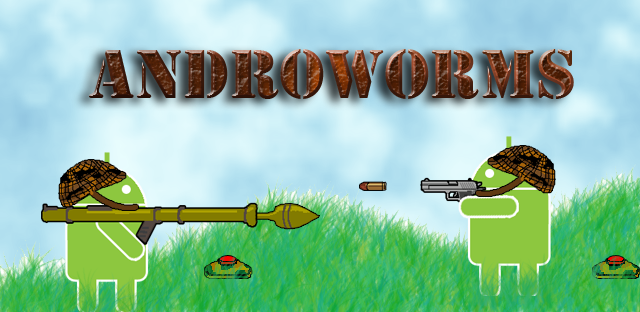
\includegraphics[scale=0.8]{images/splash}

\end{center}
\vfill
\newpage
%\vspace{10mm}
\tableofcontents
\newpage

\section{Introduction}
Les projets de jeux vidéos sont souvent mal estimés. Bon nombre de personnes pensent que c'est un jeu d'enfant de créer un jeu et pourtant cela est rarement le cas. Certains développement de jeux vidéos peuvent présenter des aspects plus complexes que des programmes basiques. En effet, il faut constamment faire attention à ne pas utiliser toutes les ressources disponibles : la partie graphique et les performances techniques étant généralement plus gourmands que pour des programmes normaux. De plus, les ralentissements dans le jeu imputent fortement la jouabilité, ce qui dérangera l'utilisateur final. La gestion des ressources représente donc un des objectifs principal du projet.
\bigskip

Pour ce projet, nous avons décidé de mettre l'accent sur les quatre objectifs ci-dessous :
\begin{itemize}
\item l'ergonomie : une GUI facile à utiliser
\item la jouabilité : un jeu simple et fonctionnel
\item les performances : un temps de réponse très faible et pas de latence 
\item le caractère innovant du projet
\end{itemize}

\section{Choix du sujet}

\subsection{Nos spécifications}

Le choix d’un projet mobile s’est imposé pour plusieurs raisons. 
En effet, ce projet nous est apparu comme une occasion de découvrir le développement sur smartphone ; aucun membre du groupe n’ayant eu l’occasion d'effectuer de développement mobile jusque là. De plus, ces cinq dernières années, l'essor des smartphones a quelque peu bouleversé le marché des logiciels informatiques en plaçant le mobile en première place et rendant le développement mobile un métier d’avenir.
L’acquisition de nouvelles compétences, nous a décidé à relever ce challenge : découvrir la programmation mobile à travers ce projet. 
Aucun membre de l’équipe n’ayant de smartphone sous Windows Phone ou iOs, le choix du système d’exploitation s’est rapidement tourné vers Android. Pour des raisons budgétaire, il n’était pas envisageable d’acquérir de nouveaux matériaux.
Au final seul Renaud, ne disposant pas de smartphone ou tablette, a du utiliser intégralement la machine virtuelle Android pour réaliser ses développements et tests.

Les spécifications issus du cahier des charges et utilisés dans notre application sont les suivantes :
\begin{itemize}
\item un développement Java
\item un développement uniquement sous Android 
\item un jeu de plateforme s’appuyant sur le célèbre jeu “worms”
\item la possibilité de jouer en multi-joueurs
\item l’utilisation des capteurs des smartphones
\end{itemize}

\subsection{Vos spécifications}
Lors de la définition de notre projet, nous avons compris que l’objectif de ce projet était de faire un site internet ou une application mobile selon le travail effectué en entreprise. Nous sommes plusieurs dans le groupe à participer à la création de sites web dans le cadre de notre travail, c’est pourquoi nous avons choisi Android, que nous n’avons jamais utilisé, afin de respecter l’objectif du projet.

Nous avons également compris que vous attentiez à ce qu’on l’on fasse un projet sur un sujet inconnu avec de réelles contraintes techniques. A travers ce projet, nous avons du mettre en avant nos capacités d’adaptation et de prises de décision pour réussir à atteindre nos buts malgré les difficultés. En effet, l’intégration des API sociales pour pouvoir partager le score des joueurs a été un réel challenge que nous développerons dans la suite du rapport..

Dans cette optique de travail, nous nous sommes intéressés aux capacités techniques de nos appareils, en utilisant les capteurs du téléphone comme la caméra, le touch et multi-touch sur l’écran, le son, le vibreur et l’accéléromètre.

Lors de la démonstration de mi-projet, vous nous avez suggéré l’utilisation de SDK pour nous aider dans la conception de ce projet. 
Malgré cette demande, cela n’a pas pu être réalisé pour plusieurs raisons :
\begin{itemize}
\item l’utilisation des composants graphiques internes à Android représentaient déjà un véritable challenge pour nous
\item il existe peu de SDK pour les applications Android 2.3.x et plus
\item il faut beaucoup de temps pour comprendre et apprendre à utiliser un SDK. Ce temps rajouté à l’apprentissage d’Android, aurait représenté une part trop importante de notre projet.
\item un nouvel outil, c’est également plus de difficultés et des bugs à prévoir, mais aussi des limitations d’usage qu’on peut rencontré en cours d’utilisation.
\item le SDK n’aurait pas répondu exactement à nos demandes
\item nous avons choisi de découvrir Android tel quel sans sur-couche dans le cadre de ce tout premier projet d’application mobile
\end{itemize}

\section{Analyse du sujet}

\subsection{Moyens techniques}

\subsubsection{Choix du langage et de l'API}

Pour notre premier projet Android, nous avons décidé d’utiliser le SDK Android (Java) version 2.3.X afin d’obtenir une compatibilité avec la majorité des appareils android enregistrés à ce jour, c’est à dire 84,2%.

Cependant, entre septembre début du projet et juin, l’état du marché a énormément bougé.
Plus de 50\% des mobiles utilisent actuellement une version 4.0.X ou supérieur, ce qui ne justifierait plus forcément notre choix de départ.
Ceci s’explique par une technologie relativement récente entraînant la sortie de mises à jour fréquentes et surtout la venu de nombreux mobiles rendant les vieilles versions obsolètes. 

L’anticipation de cette évolution et l’utilisation de la version 4.0.X et de son API nous aurait grandement simplifié le développement. Dorénavant, le développeur n’est dorénavant plus obligé de tout redévelopper de lui même, de qui engendre un gain de temps phénoménal.
\bigskip

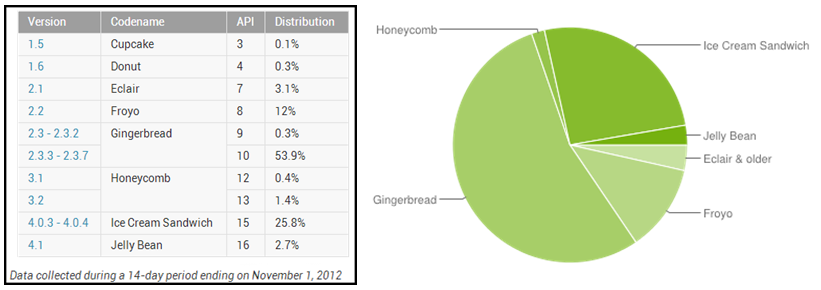
\includegraphics[scale=0.75]{images/graph1}

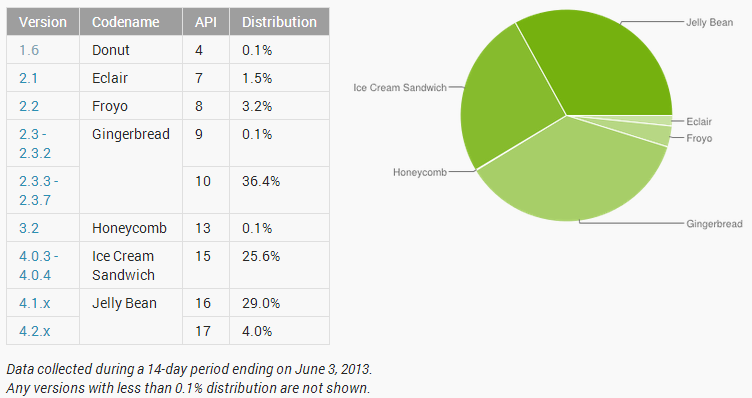
\includegraphics[scale=0.75]{images/graph2}

\subsubsection{L'environnement de développement}
Afin d’uniformiser l’environnement de développement entre tous les membres de l’équipe, une documentation d’installation et configuration de l’IDE et des plugins a été créée.
D’un commun accord, il a été décidé d’utiliser eclipse que ce soit sous Windows ou Linux, auquel on a rajouté le SDK Android et le plugin du gestionnaire de version.

\subsubsection{Le gestionnaire de version}

Afin de rendre le code source disponible, nous avons décidé de l’héberger sur google code à l’adresse suivante : http://code.google.com/p/androworms/
Ce choix nous a permis d’utiliser le tracker intégré, permettant d’affecter des tâches aux différents membres du groupe, que ce soit pour des bugs ou des demandes d’évolutions (http://code.google.com/p/androworms/issues/list). Cette fonctionnalité permet l’envoie direct d’un mail à la personne en charge de la tâche.

N’ayant jamais eu de problème de compatibilité entre eclipse et SVN, son choix comme gestionnaire de version s’est rapidement imposé.

\subsubsection{La gestion de la qualité}

Dès le début du projet, Sonar a été installé sur le serveur tiers afin de contrôler et améliorer la qualité du code source.
Cette plate-forme de contrôle continue, effectue une analyse à chaque commit et renvoie le résultat en moins d’un minute.http://doc.petrolkiwi.net/

Un code propre et facile à maintenir est absolument nécessaire, essentiellement lorsqu’on est plusieurs à intervenir dessus. En effet, il n’est pas toujours évident de comprendre le code des autres, mais cela peut être encore plus contraignant si le code n’est pas propre ou correctement indenté.

(et lien à la fin de la bibliographie du site de l’aius, du site principal de sonar)

\subsubsection{Communication}

La communication au sein du groupe n’a pas toujours été facile. Principalement en raison de l’emploi du temps de chacun, mais également en raison de la division par groupe pendant les td/tp. Au final très peu de travail personnel en commun.

D’autres moyens de communications ont été utilisés :
\begin{itemize}
\item Des mails, plus de 250 à chaque fois adressés à toute l’équipe.
\item La création d’issue tracker individuel.
\item Des commentaires sur les commits sous forme de mails individuels.
\item Des réunions pour les grosses décisions : rédaction du cahier des charges, élaboration de la vidéo finale, etc...
\end{itemize}

\section{Moyens techniques mis en place}

Réunion pour la définition du sujet et des limites (fonctionnalités minimales et maximales)
Choix des technologies employées (version du SDK et technologie réseau )
\bigskip

Répartition des taches:

\begin{tabular}{|c|c|c|c|c|c|c|c|}
\hline
{\bf Tâche } & {\bf William } & {\bf Audrey } & {\bf Damien } & {\bf Marie-Hélène } & {\bf Renaud } & {\bf Avancement}\\
\hline
{IHM des menus} & {} & {} & {X} & {} & {} & {90\%}\\
\hline
{IHM du jeu} & {} & {} & {} & {} & {} & {}\\
{(graphismes)} & {} & {X} & {} & {} & {} & {88\%}\\
\hline
{IHM du jeu} & {} & {} & {} & {} & {} & {}\\
{(gestion des composants)} & {} & {X} & {X} & {X} & {} & {80\%}\\
\hline
{Editeur de carte} & {X} & {} & {} & {} & {} & {92\%}\\
\hline
Déplacement des perso &&&&&&\\
(déplacement + &&&&& X&76\%\\
gestion de la collision + &&&&&&\\
 gravité) &&&&&&\\
\hline
{Armes (trajectoire)} & {} & {} & {} & {} & {X} & {98\%}\\
\hline
{Jeux tour à tour} & {X} & {} & {} & {} & {X} & {90\%}\\
\hline
{API (Facebook,} & {} & {} & {} & {X} & {} & {90\%}\\
{ Google+, Twitter)} & {} & {} & {} & {} & {} & {}\\
\hline
{Gestion du réseau} & {} & {} & {X} & {X} & {} & {90\%}\\
{(Bluetooth)} & {} & {} & {} & {} & {} & {}\\
\hline
{Intelligence Artificielle} & {} & {} & {} & {} & {X} & {10\%}\\
\hline
\end{tabular}
\bigskip


Mise en place du dépot google.
Mise en place de convention de codage + sonar.

Etude du fonctionnement du SDK android (comment coder sur android)
\bigskip

Diagramme d’utilisation: \\
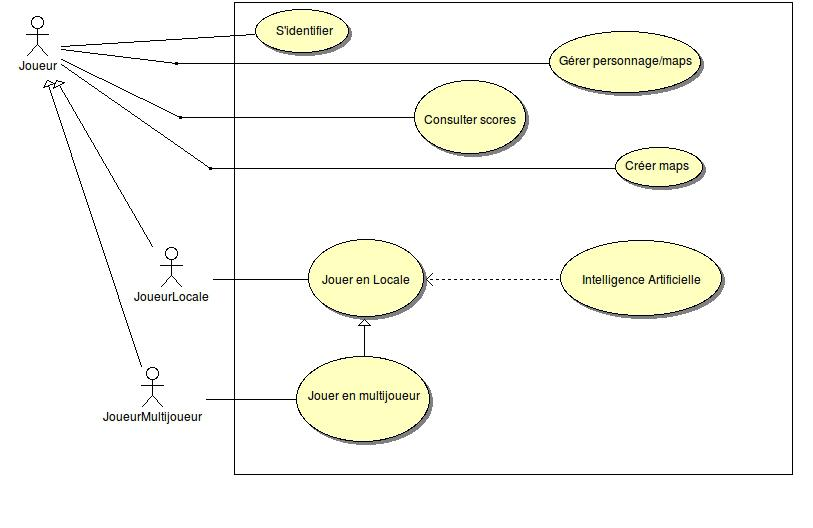
\includegraphics[scale=0.5]{images/graph3}

Elaboration d’un diagramme de classe
Lors de la spécicification du projet, un diagramme de clasess avait été construit. Ce diagramme ne comportait un nombre de classe très faible. Étant soucieux d’utiliser au une représentation UML, le premier diagramme fût enrichi pour obtenir la version suivante :\\

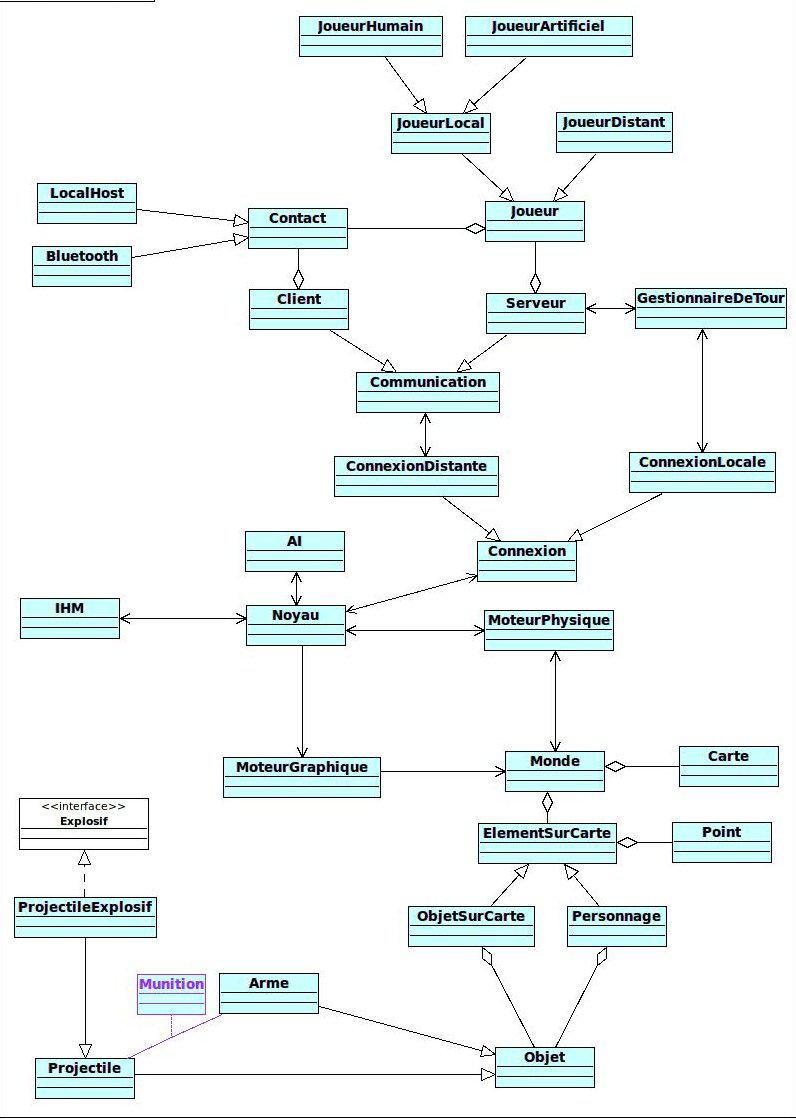
\includegraphics[scale=0.5]{images/graph4}
\bigskip

Nous ne connaissions pas les besoins de ce projet à cause de nos lacunes dans la conception et réalisation de jeu vidéo. Ce schéma a donc été notre référence pour tout le projet. La création de ce schéma a soulevé des questions importantes: 

\begin{itemize}
\item Comment faire pour garder le même comportement en solo qu’en multijoueur ?
\item Où placer l’intelligence artificiel ? Dans la partie réseau, permettant ainsi qu’elle s'exécute sur l’appareil le plus puissant ? L’accrocher au noyau pour faire simple ?
\end{itemize}

Code et correction de code

\section{Réalisations et difficultés}

\subsection{Présentation du projet}

Le but du projet était d'acquérir des compétences complémentaires à celle acquises en entreprises, d’où l’idée de créer un mini jeu mobile pour android. Ce jeu est une version modifiée du jeu bien connu Worms, dans lequel deux joueurs (ou un joueur et une IA) s’affrontent en s’envoyant des projectiles jusqu’à ce qu’un des joueurs n’ait plus de points de vie.
Pour mener à bien ce projet, nous avons découpé le projet global en sous projets articulés. Ci-dessous une présentation de ces sous projets et de leur avancement.

\subsection{Architecture du projet}

Comme précisé la section précédente, le diagramme de classe a plutôt bien guider les développements. Cependant il ne pouvait pas être précis car nous ne connaissions pas les besoins et les spécificités d’un telle projet.

La représentation de notre programme n’a pas été modifié pendant un long moment et voici le diagramme de classe de notre application actuelle :

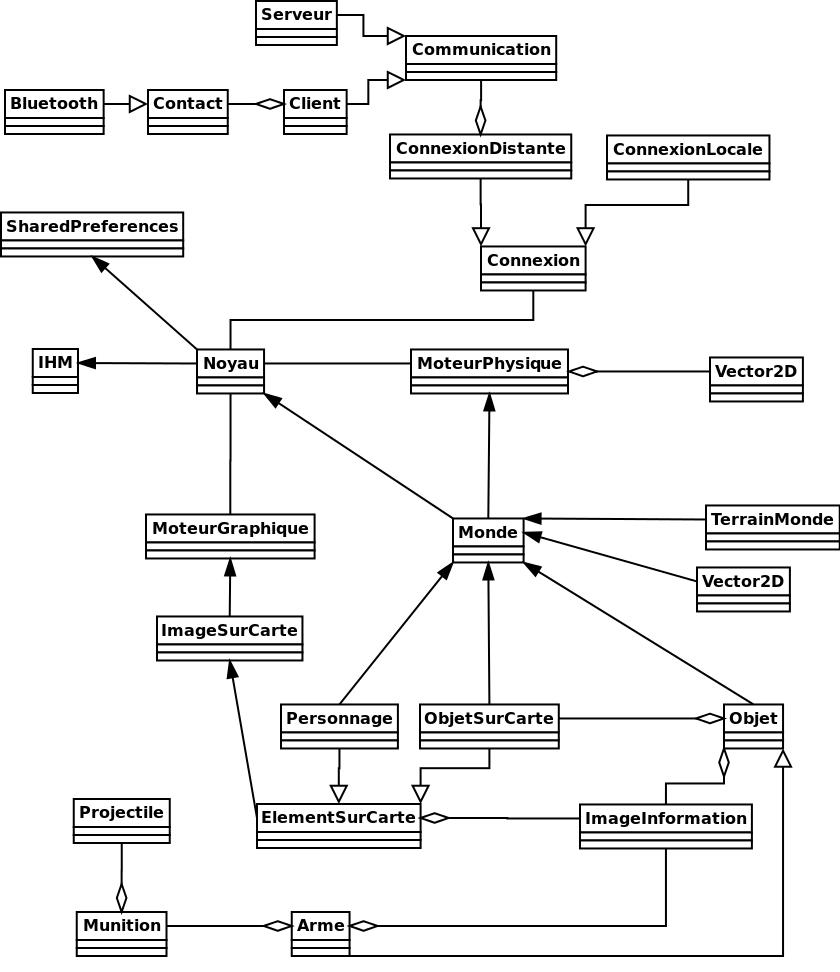
\includegraphics[scale=0.5]{images/graph5}

Dans ce schéma, les flèches noires pointent vers un objet appelant l’objet d’où la flèche part c’est de l'agrégation. Les losanges blancs indiquent la composition et les traits indiques de l’agrégation dans les deux sens. 
On remarque que le diagramme de classe initial à bien été respecté. Il y a cependant quelques erreurs qui s’y sont glissé. Par exemple, la classe “ImageSurCarte” n’est utilisé que pour stocker les informations du “Personnage” pour permettre son affichage. Il est possible de fusionner les deux classes et de garder une seule et unique classe “Personnage” qu’il faudra allé chercher via le noyau.
La classe “TerrainMonde” a remplacé la classe carte, pour deux raisons :
\begin{itemize}
\item Une autre classe “Carte” a été créée est correspond mieux à la dénomination ;
\item La classe “TerrainMonde” répresente plus qu’une simple car on peut y trouver l’arrière plan, le premier plan et le terrain constitué des deux premiers items pour éviter de recréer la map à chaque calcul.
\end{itemize}
L’une des grosses difficultés fût de comprendre le fonctionnement d’une interface fin d’y inclure des animations. Les animations posent des soucis car il faut redessiner l’écran sans interventions de l’interface graphique ou de l’utilisateur. Pour les mouvements, cela est assez simple, l’interface graphique invoque des méthodes, les modifications sur la position du personnage sont faite. Ensuite on demande l’actualisation de l’interface et notre code s’arrète. Là les appels sont dépilés et c’est parce qu’ils sont dépilés qu’il y a une réactualisation de l’interface. Notre soucis était d’utiliser ce mécanisme afin d’obtenir une animation. Ne le connaissant pas a priori, nous étions parti sur des threads, puis sur des activités, peine perdu.

Le plus simple fut d’utiliser des classes “Runnable” mais pas de façon traditionnelle. Les runnables sont comme des threads, et justement notre problématique est de relâcher le fils d'exécution. Les Runnables ont une gestion des messages efficaces en java et c’est ce que nous avons utilisé. Lorsqu’il fallait faire une animation, un Runnable était créé et appliquait un changement sur un personnage par exemple, puis lançait un message interne en se passant en paramètre. Le fils d'exécution était donc relâché et le mouvement d’un personnage était effectué.
Lorsque le message interne revenait, l’intégralité du fils d'exécution était restaurer, permettant donc de redessiner quelques choses dans interventions de l’utilisateur ou de l’interface graphique.

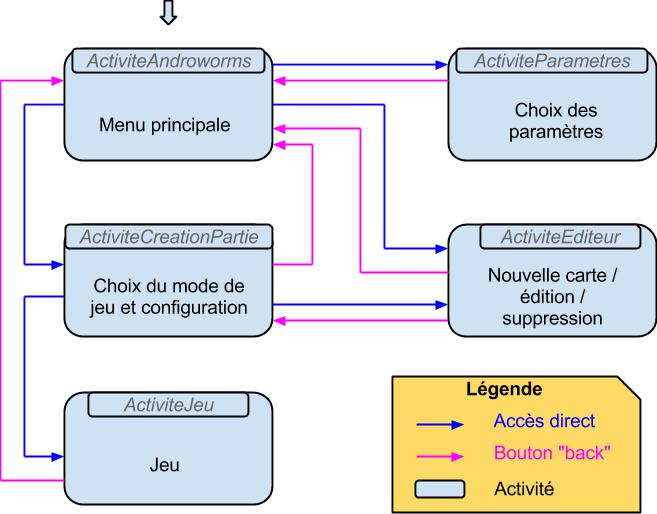
\includegraphics[scale=0.5]{images/graph6}

\subsection{La GUI}

Partie de Damien majoritairement: parler de la GUI qui reste facile d’utilisation car très intuitive et rappelant celles de nombreux jeux existants (on retrouve les boutons 1 joueurs, 2joueurs, paramètres …)

\subsection{Les graphismes}
En France, il n’est pas nécessaire de déposer une oeuvre pour qu’elle soit considéré comme telle et protégée. De ce fait, une majorité des images présentes sur internet est soumise au droit d’auteur. Ce droit protège les image de la modification, reproduction, diffusion ; elles ne peuvent être exploitées sans l’autorisation de l’auteur.
Pour des soucis de légalité et dans l’optique d’une éventuelle commercialisation de l’application dans le futur, nous avons décidé de créer nos propres images.
Chaque smatphone ayant un espace mémoire différent, il a fallut créer des images de taille respectable et utilisables sur tous les appareils. Une image de taille trop importante serait trop longue à charger sur certains téléphones et pourrait créer des erreurs OOM (mémoire insuffisante) en prenant trop de place en mémoire.

Concernant le déplacement des personnages, nous avons tout d’abord pensé à utiliser des sprites, mais l’image aurait également été lourde en mémoire. De plus, Android propose une propriété Animation sur les View, permettant d’enchainer plusieurs images à la vitesse choisie.

\subsection{Le jeu et la physique}

\subsubsection{Les collisions}
La gestion des collisions a subit un grand changement dans son fonctionnement.
Dans les premières versions d’androworms, l’accent avait été mis sur les performances limitées des devices. C’est pourquoi la gestion des collisions devait représenter un calcul très important. La première version de collision utilisait des enveloppes convexes afin de les gérer. C’est un système bien plus rapide que de parcourir l’ensemble des points du personnage pour vérifier les collisions. Notre bonhomme faisant 81x107 pixels (8667pixels en tout) et à chaque pixel de déplacement cette vérification doit être faite. Le soucis de l’enveloppe convexe se pose lors des sauts, où dans ce cas les déplacement ne se limite pas à un pixel de coté. Peut de temps après, le système d’enveloppe convexe a été mis de coté pour un calcul exhaustif de la collision afin de pallier à toutes les possibilités.

\subsubsection{Les déplacements}

Les déplacements utilisent le système de collision détaillé un peu plus haut et un joueur ne peut se déplacer, marcher, uniquement si la différence de la hauteur des positions est inférieur a un certain seuil fixé.

\subsubsection{Les sauts et les tirs}
Les sauts et les tirs suivent la même mécanique, la seule différence est les valeurs initiales. Pour les sauts, le vecteur initial est fixe et défini dans l’application, alors que pour les tirs, c’est au joueur de définir le vecteur d’initialisation. Ensuite chaque point de la trajectoire est calculé, puis stocké et ensuite fait l’objet d’un affichage. Pour la trajectoire, un intervalle de temps fixe est choisi (pour l’instant 200ms) et chaque point est calculé a partir du point initial et du temps écoulé.
L’équation pour une position est la suivante :

$
x = P_{x} + t*V_{x} + \sum t^{2}* a_{i}
$

\bigskip

Avec :
\begin{itemize}
\item P: la position initiale
\item t: un temps donné,
\item V: un vecteur initial 
\item a: un tableau d’accélération (typiquement la gravité et le vent)
\end{itemize}

\bigskip

Pour la position suivante nous avons :

$
x = P_{x} + (t+\epsilon)*V_{x} + \sum (t+\epsilon)^{2}* a_{i}
$
\bigskip

Avec :
\begin{itemize}
\item P: la position initiale
\item t: un temps donné,
\item V: un vecteur initial 
\item a: un tableau d’accélération (typiquement la gravité et le vent)
\item $\epsilon$: le quantum de temps choisi
\end{itemize}

Les positions en y se calculent exactement de la même manière. 
Pour la gravité, il va de soi, que le vecteur initial est nul, seul les accélérations entre en compte. 

D’ailleurs pour ce genre d’action, il faudra faire attention à ce que le saut, la gravité ou le tir s'arrête bien lorsqu’il rentre en contact avec les éléments du décor. En effet, l’action suit une somme de quantum de temps, mais lorsque cette somme est grande, la nouvelle position est à K pixels de la précédente (K >= 1). Sur la fin de la trajectoire il y aura que peu de chance que le personnage effectuant un saut arrive les deux pieds par terre. Il flottera sûrement dans les air car c’est ici que se situait la dernière position valide n’impliquant pas la collision. Il faudra ajuster la position en fonction des deux derniers points (l’avant-dernier point valide et le dernier point invalide). Pour pallier à ce problème, notre code parcourt l’ensemble des points formé par la droite décrite par ces deux derniers points et en déduit la position réel de l’élément.
Ce fonctionnement rends la position réel imprécise car les accélérations produisent généralement une trajectoire “bombée”. Cette imprécision est acceptable pour l’application que nous développons.

\subsection{Le réseau}

parler des études de technologies que nous avons faites à notre première réunion
(WIFI == overkill, IR impossible, Bluetooth bon compromis)

\subsection{Générateur de cartes}

Un des caractère innovant de cette application est sans nul doute le
générateur de cartes.
En effet, aucun autre jeu de type worms que nous avons trouvé dans le
store ne permettait de générer ses propres cartes. Pour cela, nous avons
pensé une application pouvant prendre des photos, et permettant de jouer
dessus, selon le même principe que la réalité augmentée mais en version
statique.

Au début, nous voulions juste utiliser l'image en fond et rajouter
par dessus l'image de la terre sur laquelle les joueurs se poseraient.
Puis, après discussion, nous avons trouvé qu'il serait plus amusant
de considérer l'image en tant que sol et qu'on puisse la détruire avec
les impacts des armes.

On à donc implémenté la possibilité d'utiliser la caméra intégrée pour prendre des photos.
Cette étape qui devait être simple s'est avérée être en fait bien plus compliquée que prévu.
En effet, les informations publiées dans la documentation de l'API android
n'est pas respectée. Lors de l'appuie sur le bouton pour prendre une photo,
un callback est appelé lorsque l'image est disponible en format dit "raw" et
est transmis en argument,
puis un autre est appelé un peu plus tard lorsque l'image est disponible en
format compressé jpeg et le transmet en argument. Mais dans les nouvelles version d'android, ces callbacks
sont toujours appelés pour des raison de rétro-compatibilité, mais le callback
d'image "raw" est appelé en envoyant null comme argument. Alors que nous voulions
utiliser un format "raw" pour choisir le format, la compression des données,
les données brutes n'étaient jamais disponibles. Aucune documentation
ne spécifiait que dans les dernières versions d'android, aucune image
brute n'était plus disponible. Nous avons donc utilisé les images déjà
compressées.

L'étape suivante était d'implémenter la possibilité de dessiner sur l'image
ou sur un fond bleu de la terre, et d'effacer de la terre pour remettre du ciel.
Le plus intuitif selon nous pour faire celà était d'utiliser de la transparance,
les zones transparantes représentant le ciel, et les zones non transparantes
représentant la terre. Nous avons décidé d'utiliser plusieurs tailles
de brosses afin de faire des dessins plus ou moins précis. Lors d’un appui sur l’écran, nous dessinons alors un cercle dont la taille dépend de la taille de brosse choisie, et nous le colorions en couleur terre, puis nous colorions le tour du cercle en couleur herbe, ou alors nous appliquons une transparence si l’outil d’effacement est sélectionné.

Lors des tests, nous nous sommes aperçus que pendant le temps de traitement durant lequel nous dessinions le cercle et appliquions les transformations, l’application était bloquée et ne répondait plus aux actions de l’utilisateur. une des conséquences et que nous n’obtenions pas de traits continus lorsque l’on effectuais un glissé sur l’écran. Dès lors, une de nos priorité à été de traquer les moindres ralentissements de l’application lors du dessin, ce qui fût une tâche difficile et longue.

La dernière chose que nous avons implanté, c’est un algorithme permettant à l’utilisateur de séparer automatiquement la photo en zone de ciel et zone de terre. Cette fonctionnalité permet en effet de sélectionner les zones claires, et d’appliquer de l’alpha dessus afin de les transformer en ciel. Pour cette fonctionnalité, plusieurs algorithmes on été essayés.

Seuillage fixe:
On choisit une valeur de densité que l’on appel seuil, puis on parcours l’image en calculant la densité de chaque pixel. Si cette densité est inférieure à la valeur de seuil, le pixel sera transformé en ciel, et si la densité du pixel est supérieure au seuil, le pixel sera conservé tel quel.

Cet algorithme à l’avantage d’être simple et peu coûteux en temps et ressources, mais les résultats produits étaient très aléatoires et peu esthétique. Notamment qu’on ne peut prédire si l’image sera plutôt claire ou plutôt sombre, si le seuil choisit est trop bas et que l’image est sombre, la carte ne contiendra pas assez de ciel et les personnage ne pourront pas se déplacer. Si au contraire le seuil choisit est trop haut et que l’image est claire, la carte finale ne contiendra pas de terre et les personnages tomberont instantanément.

Seuillage dynamique.
On procède tout d’abord à un calcul de la densité moyenne de l’image. Cette densité moyenne indiquera au programme si l’image est plutôt sombre ou plutôt claire. Nous prenons alors cette densité moyenne pour valeur de seuil et utilisons alors la même technique que dans l’algorithme précédent.

Cette technique est très peu coûteuse mais ne donne pas de résultats très esthétiques.

K-means:
On débute en prenant deux pixels aléatoire p1 et p2, on calcul leurs densité d1 et d2. Ces deux densités forment alors la base de deux ensembles e1 et e2. On parcours ensuite l’ensemble des pixels, et pour chaque pixel p, on calcule sa densité d, et en le place dans un des ensemble selon le critère suivant:
	-si la distance |d-d1| est inférieure à la distande |d-d2|, on le placera dans l’ensemble e1.
	-si la distance |d-d1| est supérieure à la distande |d-d2|, on le placera dans l’ensemble e2.
Une fois tous les pixels de l’image parcourus, on calcule la densité moyenne de chacun des pixels appartenant aux ensembles, d1’ et d2’. Ces deux densité servent alors de base à deux nouveaux ensemble e’1 et e’2. On réitère un nombre fixe de fois jusqu’à obtenir deux densité moyennes finales f1 et f2. La plus faible de ces densité sera prise pour densité du ciel et la plus élevée sera prise pour densité de la terre. On regroupe alors de la même façon que précédemment les pixel selon si leur densité est plus proche de la densité du ciel ou la densité de la terre. On applique enfin un alpha aux pixel dont la densité est plus proche de la densité du ciel.

Cet algorithme donne de bons résultats quel que soit le type de photo, mais est extrêmement coûteux en temps, surtout sur du matériel possédant un faible processeur.

Technique hybride
D’après les tests effectués sur les autres algorithmes, nous avons alors imaginé un algorithme hybride essayant d’allier des résultats esthétiques et peu coûteux.
L’algorithme imaginé sépare les pixels de l’image en deux classes, la classe du ciel et la classe de la terre à la façon de l’algorithme K-means (celui qui donnait les meilleurs résultats). Nous partons de l’hypothèse que le ciel est plus clair que la terre. On effectue un premier parcous de l’image en cherchant le point le plus clair (le moins dense) et le point le plus sombre (le plus dense) de l’image. Nous séparons ensuite les pixels de l’image en deux classes : la classe sombre et la classe claire, de la même façon que l’algorithme K-means, en calculant la distance entre la densité de chaque pixel et les points sombres ou clairs. Puis nous appliquons de l’alpha sur les points les plus clairs.

Cet algorithme était beaucoup moins coûteux que K-means et donnait des résultats semblables.
Cependant, on pouvait observer des artefacts: certains pixels clairs qui apparaissaient au milieu de zones sombres se voyaient appliquer un alpha, ce qui donner des résultats peu esthétiques. Pour l’améliorer, nous avons décidé de diminuer la résolution de calcul. Lors de la phase de séparation, au lieu de traiter pixel par pixel, nous traitons des blocs de plusieurs pixels, calculant la moyenne de densité des blocs avant de les classer dans l’une ou l’autre des catégories.


C’est ce dernier algorithme que nous utilisons car il donne des résultats très esthétiques avec un temps de calcul suffisamment réduit.


%
%Status : Terminé mais pas complètement intégré.
%Fonctionnalités:
	%Prise de photo
	%Choix de taille de brosse
	%Ajout de ciel
	%Ajout de terre
	%Enregistrement de la carte (avec choix du nom)
	%Seuillage automatique (très bons résultats sur images avec fort niveau de contraste)
%
%Limitations : 
%pas d’annulation des actions possible == problème de mémoire

\subsection{Problèmes rencontrés et solutions appliquées}




\end{document}
